\clearpage
\subsection{太陽電池の発電特性の実験}

\subsubsection{太陽電池の発電特性の実験器具}
使用した実験器具を\wtab{kigu4}に示す.
\begin{table}[h]
  \centering
  \caption{実験装置}
  \label{tab:kigu4}
  \scalebox{0.7}{
  \begin{tabular}{cccccc}
	\hline
	機器名&製造元&型番&シリアル番号(または管理番号)\\
	\hline
	太陽電池&SUNYO&SY-M5W&-\\
	ディジタル照度計& Zhangzhou Weihua Electronic Co., Ltd&LX-1010B&T 428585\\
	ディジタル温度計&Gain Express Holdings&THE-27 Digital Thermometer 4 Channel K-Type&202019031\\
	ディジタルマルチメータ&owon&B35&B351518443\\
	可変抵抗器&TOKUSHU DENKI KOGYOSHO&S-3&3201\\
	\hline
  \end{tabular}
}
\end{table}

\subsubsection{太陽電池の発電特性の実験方法}
\begin{enumerate}[(1)]
	\item \wfig{solar-cell}のように回路を構築する.
	\begin{figure}[h]
	\centering
	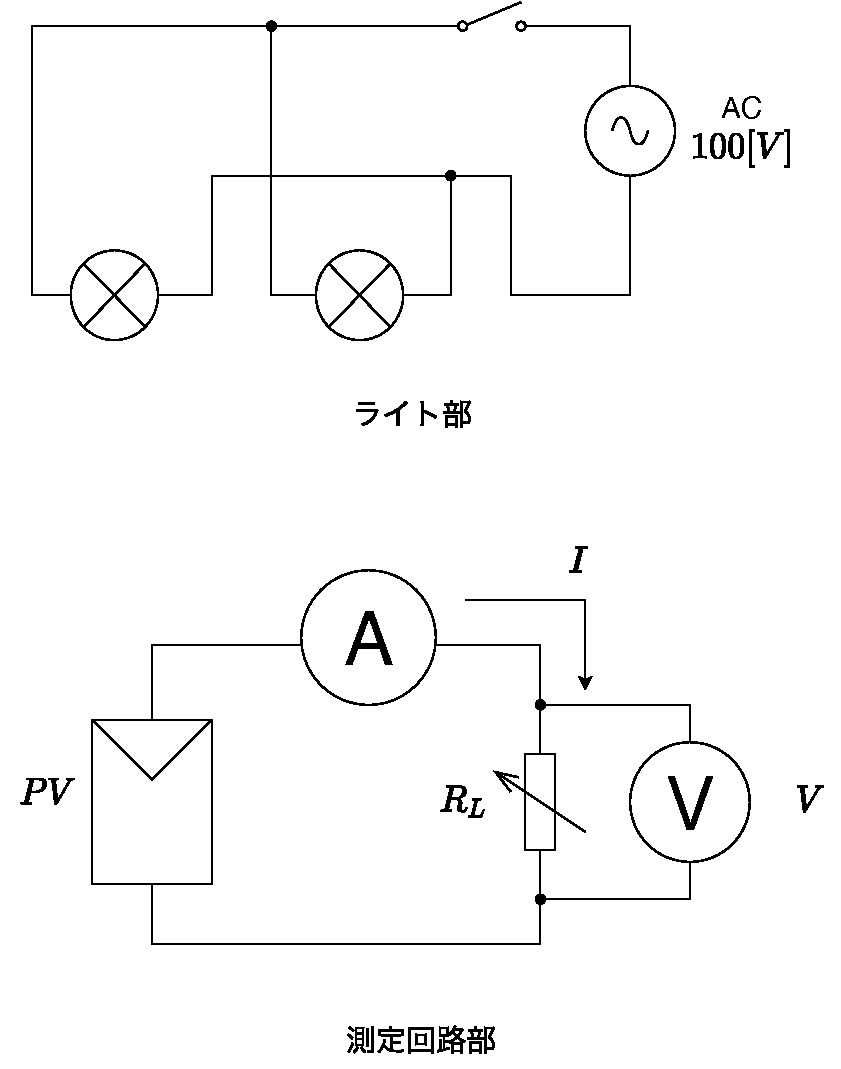
\includegraphics[scale=0.5]{./fig/solar-cell.pdf}
	\caption{太陽電池の計測回路}
	\label{fig:solar-cell}
	\end{figure}
	\item 太陽電池はライトの光が均等に照射されるように配置した.
	\item 可変抵抗器のレバーを短絡側にセットし,ライトを2つ点灯させた.
	\item 太陽電池を動かし,電流が最大になる位置を探し位置に印をつけた.
	\item ライトを1つ点灯に変更した.
	\item 太陽電池の四隅と中央の計5ヶ所に関して計測を行い.その平均値を代表値として,算出した.
	\item 太陽電池の裏面中央に温度計を設置した.
	\item 照度測定後,太陽電池温度が$30^{\circ}$Cになるように調節を行った.\label{ondo}
	\item $V-I$測定を開始した.可変抵抗$R_{L}$を変更させながら,電流$I$,電圧$V$を記録する.$V_{oc}$付近ではデータ取得間隔を細かくした.\label{I-V}
	\item 測定の際温度は$\pm 2^\circ$Cの範囲で計測を行った.
	\item 点灯させるライトを2つに変更し,上記と同様((\ref{ondo}) $\sim$ (\ref{I-V}))に計測を行った.
	\item 太陽電池温度を$50^{\circ}$Cに変更し,点灯させるライトを1つ,2つの場合に対し測定を行った.
\end{enumerate}

\subsubsection{太陽電池の発電特性の結果}
\label{solar-cell-result}
\begin{itemize}
	\item $30^{\circ}$C,ライト1つ・2つ,$50^{\circ}$C,ライト1つ・2つの計4条件での計測結果を\wtab{30-one}$\sim$\wtab{50-two}に示す.
	上記データをもとに作成した,$V-I$カーブを\wfig{VIc}に示す.
	
	これらより電流が多く流れることに関わる因子の影響は,太陽電池温度ではなく,ライトの個数(照度)の方が大きいことがわかる.また,出力される電流の最大値は決まっており,ある電圧を超えるとほぼ一定であった電流値が減少に変化することが確認される.
	そして,その電圧の値は4条件で大きく違いがなかった.
	\item \weq{power}をExcelを用いて算出した電力を用いて作成した$V-P$カーブを\wfig{VPc}に示す.
	\begin{equation}
		P=VI
		\label{eq:power}
	\end{equation}
	\begin{table}[p]
	\begin{tabular}{cc}
	\begin{minipage}[t]{0.5\hsize}
	\centering
	\caption{$30^{\circ}$C ライト1つの場合(照度8600\,\rm{lux})}
	\label{tab:30-one}
	\scalebox{1.0}{
	\begin{tabular}{ccc}
	\hline
	電圧$V$[\rm{V}] & 電流$I$[\rm{mA}]   & 電力$P$[\rm{W}] \\
	\hline
	0.8  & 63.8 & 0.1 \\
	2.8  & 63.7 & 0.2 \\
	3.5  & 63.0 & 0.2 \\
	7.0  & 63.1 & 0.4 \\
	9.8  & 62.6 & 0.6 \\
	12.3 & 62.3 & 0.8 \\
	14.3 & 61.9 & 0.9 \\
	16.7 & 61.5 & 1.0 \\
	17.3 & 60.0 & 1.0 \\
	18.3 & 56.5 & 1.0 \\
	18.7 & 50.2 & 0.9 \\
	18.9 & 45.3 & 0.9 \\
	19.2 & 40.5 & 0.8 \\
	19.4 & 35.3 & 0.7 \\
	19.5 & 30.7 & 0.6 \\
	19.6 & 25.7 & 0.5 \\
	20.0 & 20.5 & 0.4 \\
	20.1 & 15.5 & 0.3 \\
	20.1 & 10.6 & 0.2 \\
	20.2 & 6.1  & 0.1 \\
	\hline
	\end{tabular}
	}
	\end{minipage}
	\begin{minipage}[t]{0.5\hsize}
	\centering
	\caption{$30^{\circ}$C ライト2つの場合}
	\label{tab:30-two}
	\scalebox{0.9}{
	\begin{tabular}{ccc}
	\hline
	電圧$V$[\rm{V}]   & 電流$I$[\rm{mA}]   & 電力$P$[\rm{W}]  \\
	\hline
	1.9  & 151.1 & 0.3 \\
	2.7  & 151.0 & 0.4 \\
	3.9  & 148.8 & 0.6 \\
	5.6  & 148.3 & 0.8 \\
	7.1  & 147.2 & 1.0 \\
	9.9  & 144.0 & 1.4 \\
	10.7 & 141.5 & 1.5 \\
	15.9 & 137.6 & 2.2 \\
	13.7 & 141.0 & 1.9 \\
	18.6 & 136.4 & 2.5 \\
	19.3 & 127.5 & 2.5 \\
	19.7 & 105.8 & 2.1 \\
	20.0 & 91.2  & 1.8 \\
	20.4 & 80.3  & 1.6 \\
	20.2 & 74.5  & 1.5 \\
	20.3 & 61.8  & 1.3 \\
	20.8 & 50.6  & 1.1 \\
	20.9 & 40.1  & 0.8 \\
	20.8 & 29.3  & 0.6 \\
	20.9 & 20.0  & 0.4 \\
	21.2 & 10.6  & 0.2 \\
	21.1 & 6.4   & 0.1 \\
	\hline
	\end{tabular}
	}
	\end{minipage}\\
	\begin{minipage}[t]{0.5\hsize}
	\centering
	\caption{$50^{\circ}$C ライト1つの場合}
	\label{tab:50-one}
	\scalebox{0.75}{
	\begin{tabular}{ccc}
	\hline
	電圧$V$[\rm{V}]   & 電流$I$[\rm{mA}]   & 電力$P$[\rm{W}]  \\
	\hline
	1.1  & 65.0 & 0.1 \\
	2.7  & 64.6 & 0.2 \\
	5.0  & 64.6 & 0.3 \\
	6.8  & 64.1 & 0.4 \\
	7.1  & 64.3 & 0.5 \\
	9.5  & 64.0 & 0.6 \\
	12.0 & 63.5 & 0.8 \\
	14.2 & 63.1 & 0.9 \\
	16.5 & 61.6 & 1.0 \\
	16.5 & 60.3 & 1.0 \\
	17.3 & 53.3 & 0.9 \\
	17.8 & 50.5 & 0.9 \\
	18.2 & 39.1 & 0.7 \\
	18.4 & 34.9 & 0.6 \\
	18.5 & 30.2 & 0.6 \\
	18.8 & 20.4 & 0.4 \\
	19.0 & 16.1 & 0.3 \\
	18.9 & 15.1 & 0.3 \\
	19.0 & 14.1 & 0.3 \\
	19.0 & 13.1 & 0.2 \\
	19.0 & 11.1 & 0.2 \\
	19.0 & 10.2 & 0.2 \\
	19.1 & 9.1  & 0.2 \\
	19.1 & 7.1  & 0.1 \\
	19.2 & 5.8  & 0.1 \\
	\hline
	\end{tabular}
	}
	\end{minipage}
	\begin{minipage}[t]{0.5\hsize}
	\centering
	\caption{$50^{\circ}$C ライト2つの場合}
	\label{tab:50-two}
	\scalebox{1.0}{
	\begin{tabular}{ccc}
	\hline
	電圧$V$[\rm{V}]   & 電流$I$[\rm{mA}]   & 電力$P$[\rm{W}]  \\
	\hline
	2.6  & 151.4 & 0.4 \\
	5.5  & 149.8 & 0.8 \\
	7.5  & 147.9 & 1.1 \\
	10.6 & 146.5 & 1.6 \\
	13.0 & 144.0 & 1.9 \\
	15.3 & 143.7 & 2.2 \\
	17.3 & 142.0 & 2.5 \\
	18.3 & 134.4 & 2.5 \\
	18.4 & 129.3 & 2.4 \\
	18.8 & 103.1 & 1.9 \\
	19.4 & 80.4  & 1.6 \\
	19.7 & 58.8  & 1.2 \\
	19.8 & 41.0  & 0.8 \\
	19.9 & 30.4  & 0.6 \\
	20.0 & 20.7  & 0.4 \\
	20.0 & 11.6  & 0.2 \\
	20.2 & 6.1   & 0.1 \\
	\hline
	\end{tabular}
	}
	\end{minipage}
	\end{tabular}
	\end{table}
	\begin{figure}[h]
	\begin{minipage}[c]{1.0\hsize}
	\centering
	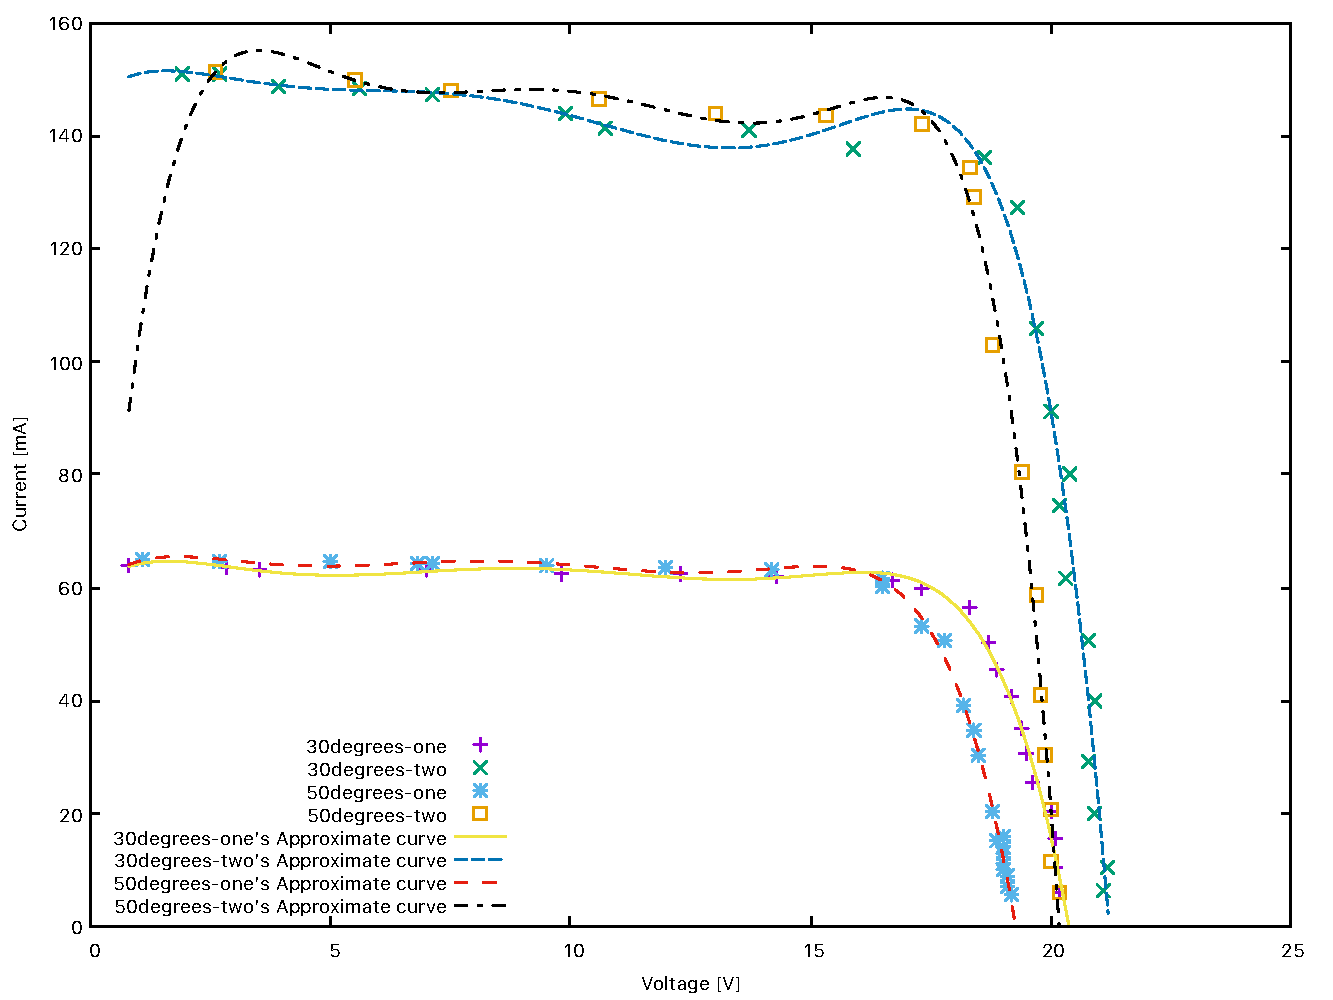
\includegraphics[scale=0.7]{./data/solar-cell/solar-cell.pdf}
	\caption{太陽電池の$V-I$カーブ}
	\label{fig:VIc}
	\end{minipage}
	\begin{minipage}{1.0\hsize}
	\centering
	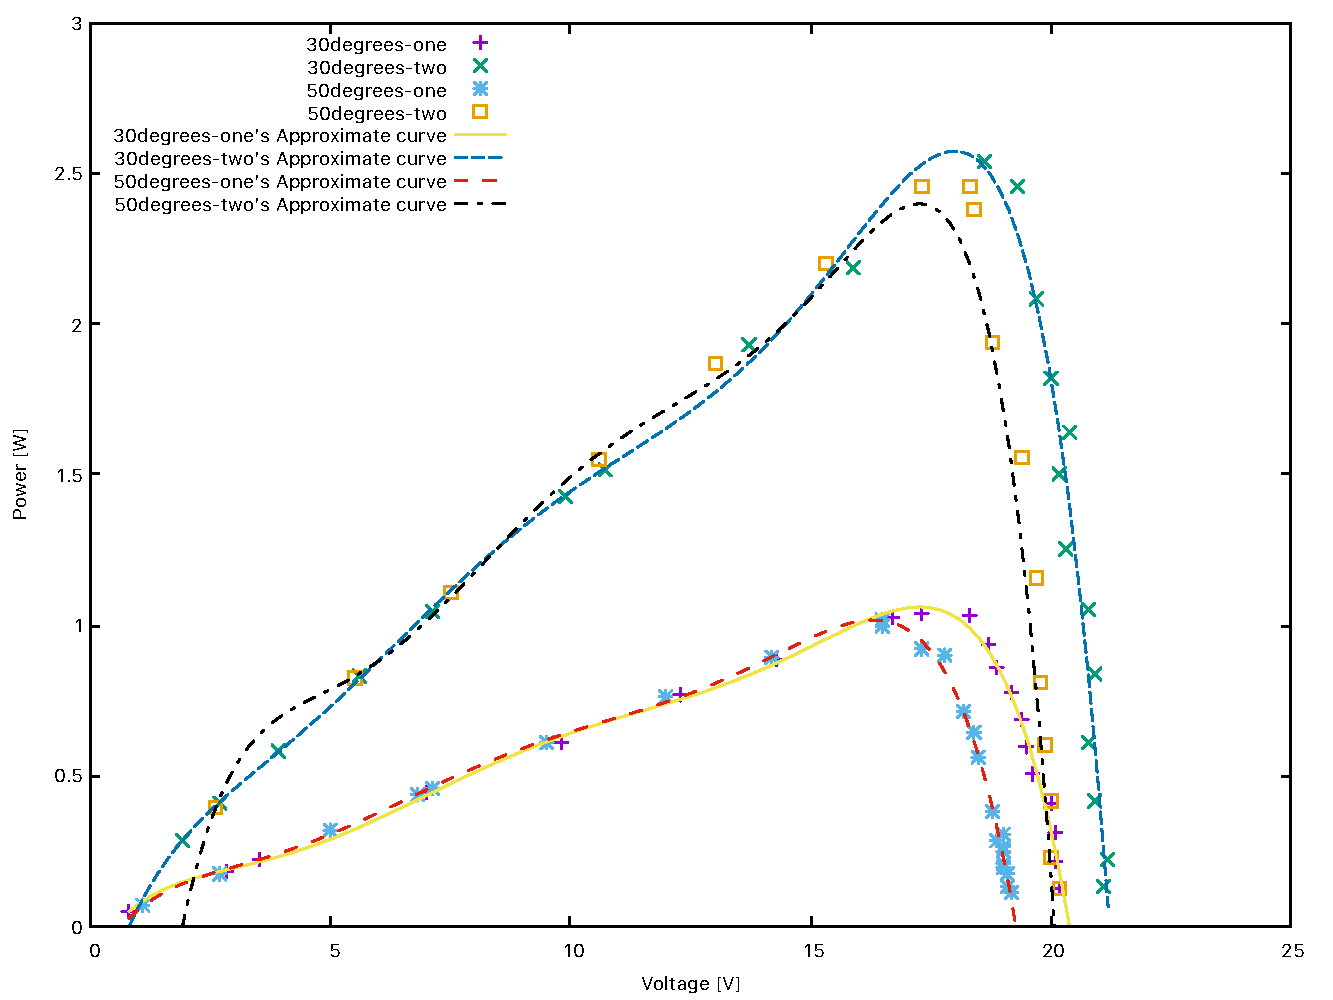
\includegraphics[scale=0.7]{./data/solar-cell/solar-cell-2.pdf}
	\caption{太陽電池の$V-P$カーブ}
	\label{fig:VPc}
	\end{minipage}
	\end{figure}
\end{itemize}

\clearpage
\subsubsection{太陽電池の発電特性の考察}
\begin{enumerate}[(1)]
	\item 各条件下の電流-電圧の測定結果から電力を算出し,$V-P$カーブを描きなさい.また,最大電力点を抽出して表にまとめ,条件の変化と最大電力点について考察せよ.
	
	$V-P$カーブは\wfig{VPc}に示した.\\
	最後に最大電流値を取る点が電力の最大点とほぼ一致していることが読み取れる.
	また,電力最大点より,小さい電圧の電流の傾きと.大きい電圧の電流の傾きは異なり,前者は緩やかで,後者は急である.
	電圧がある一定値を超えると急に電力を得ることが難しくなるとうことである.\\
	また,条件を変更しても電力最大点の移動が確認されなかったため,この点は太陽電池固有のものであると考えられる.$30^{\circ}$Cでライト2の場合つまり,低温で高い照度の場合が最も電力を多く得ることができている.\\
	電力は電流に比例し,\ref{solar-cell-result}で述べたように,電流は照度因子が温度因子より,電流に影響を与えているため,より照度が高く,太陽電池温度が低いものが電力を多く発電することができると考えられる.\\
	\weq{exp}で電流が算出できる.この式より,温度が増加すると電流が減少することが読み取れるため,上記の考察は正しいと考えられる.
	\item MPPT制御はなぜ必要か説明せよ.また,そのアルゴリズムには「山登り法」と「電圧追従法」がある.これらの特徴を調査し,比較して説明せよ.
	
	\wfig{VPc}の最大電力点で発電を行うように発電システムを構築したとしても,天候などの要因により電圧の増減し,電力が減少してしまう.そのため,最大電力点を用いた制御方法が必要となる.
	\begin{enumerate}
		\item[山登り法:] \wfig{mountan}の$P-V$曲線で電圧を一方向(増加または減少)に変化させていき,電力が増加から減少に転換すると電圧を変化させる方向を逆方向にする. これを繰り返すことにより,常に電力が最大となる最適動作点に制御する方法である\cite{esfvjsp}.
		最大電力出力点が山の頂に見え,山に登っていくように見えることからこの名前がついている.
		しかし,次に述べる電圧追従法より回路・制御が複雑であるため,コストや消費電力が高いという負の面もある\cite{nvdfsjknv}.
		\begin{figure}[h]
		\centering
		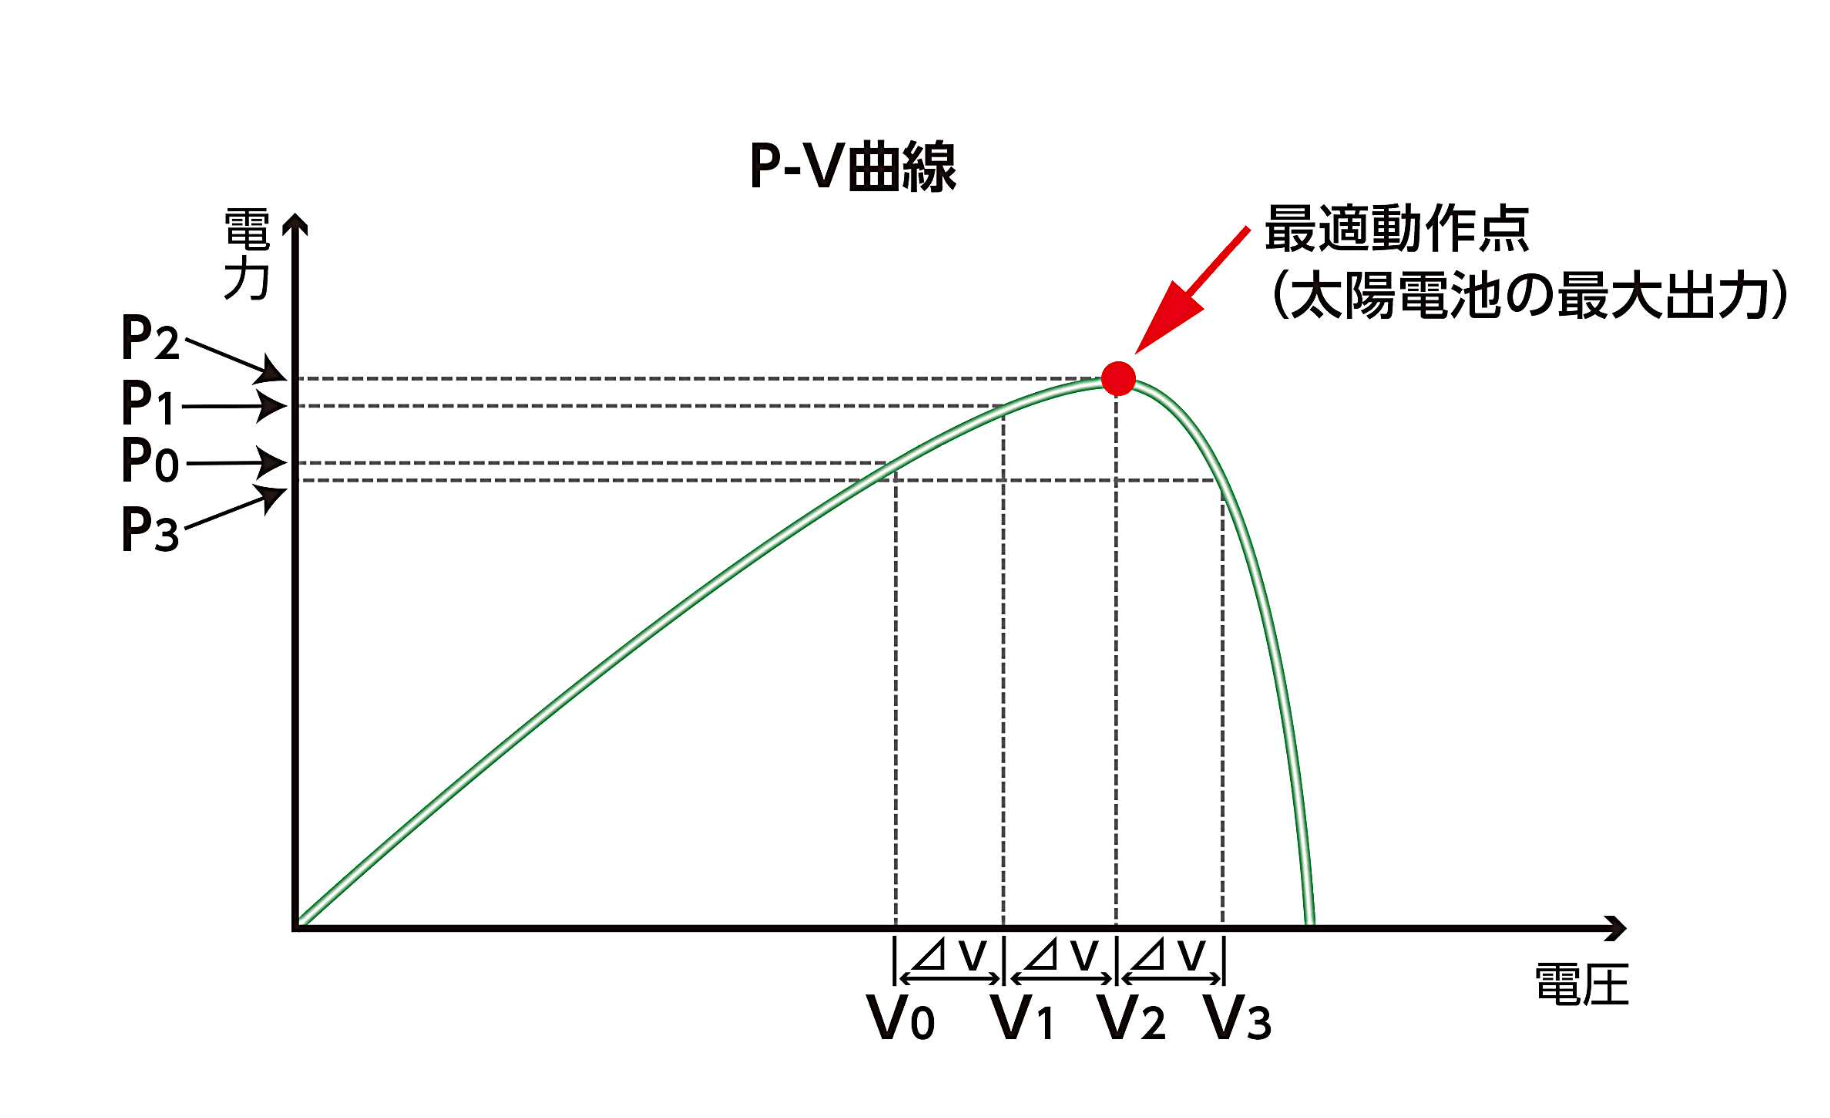
\includegraphics[scale=0.5]{./fig/mountan.png}
		\caption{山登り法\cite{esfvjsp}}
		\label{fig:mountan}
		\end{figure}
		\item[電圧追従法:]$V-I$出力特性を利用する方法である.\wfig{area}の枠の面積が発電電力を表し,$V1$のように発電電流が高く,$V2$のように発電電力が高くてもバランスが悪く,効率よく発電が行えていない状態である.しかし,$Vm$のようにそれぞれのバランスが良い状態の時,太陽電池は最大電力で発電が可能になる.この時の電圧値は開放電圧の約$80\,\%$である.
		太陽電池の動作点がバッテリーや負荷の電圧の影響を受けないため,一定の異常の効率で太陽電池から電力を取り出すことが可能である.また,電圧値の計測で制御が行えるため,容易で比較的安価であるが,気象条件により最適電圧が変動するため,最適電圧で動作していると言えない場合がある\cite{nvdfsjknv}.
		\begin{figure}[h]
		\centering
		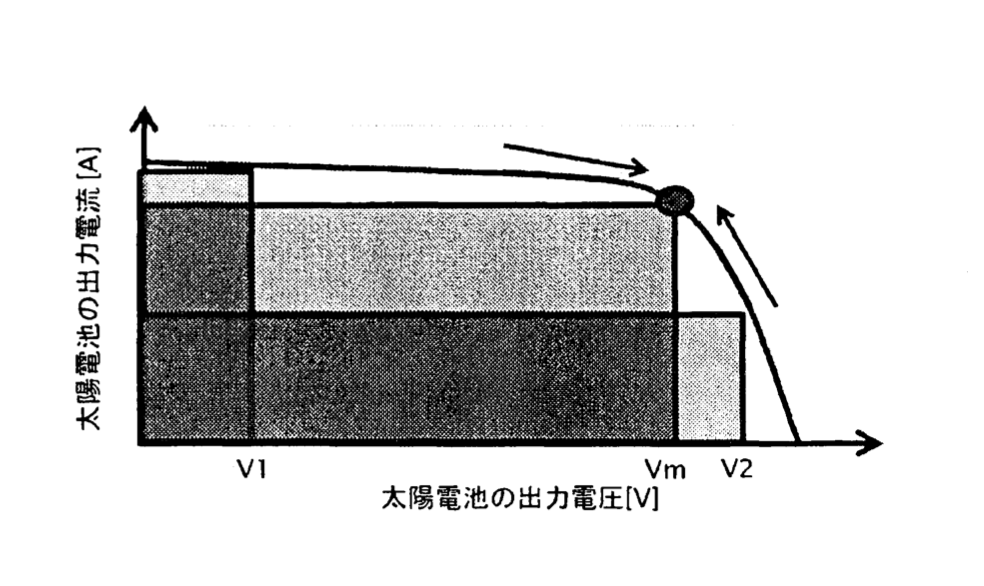
\includegraphics[scale=1]{./fig/area.png}
		\caption{電圧追従法\cite{nvdfsjknv}}
		\label{fig:area}
		\end{figure}
		\end{enumerate}
		なお,現在主流である制御方法は山登り法である\cite{main}.
\end{enumerate}